\chapter{Chapter 4 --- Experiments}\label{chapter-4-experiments}

This chapter reports the empirical results. The structure follows the framing of Chapter 3: code is the core and carries the main claims, math is a pilot that characterizes the boundary of the mechanism.

The experiments answer three questions. First, the method question (RQ-method): does the proposed teacher-first organization beat the student-first baseline at test-time discovery, and if so where and how much (§4.2)? Second, RQ1: does the reprompt template matter, and in which regime (§4.3)? Third, two robustness checks: is the result invariant to the judge choice, and does the leak ablation behave as predicted (§4.4)? Section 4.5 then reports the math pilot, which does not escape and is presented as a boundary characterization rather than a failed attempt.

A standing caveat applies to every number below. The sample sizes are small (2--3 problems for the code escape results, 2 seeds for RQ1, 2 problems for math). All significance values are \textbf{crude sign tests} of the form \(0.5^k\) over non-tied matched pairs, reported as descriptive and directional evidence, never as inferential proof. The language throughout stays at ``weak / directional dominance''; nowhere is a claim stated as ``proven.''

\begin{center}\rule{0.5\linewidth}{0.5pt}\end{center}

\section{4.1 Experimental setup}\label{experimental-setup}

\textbf{Models.} Code uses Qwen3-4B {[}7{]} with LoRA (r=32, bf16), thinking OFF. Math uses Gemma-4-E4B with LoRA on all linear layers, thinking ON. The model differs across domains, which is a confound carried explicitly into every math claim (§4.5, Chapter 6).

\textbf{Hardware.} Code runs on Colab L4 (22 GB) and A100; math runs on Modal A100-80GB (Colab compute units were exhausted).

\textbf{TTT protocol.} Per problem, the model is reset to base, then run for \(K\) steps; the student is evaluated PRE and POST with no context (§3.6). Code: \(K=15\), eval 16 samples, \texttt{teacher\_n=10}. Math: \(K=3\), eval 4 samples, \texttt{teacher\_n=4}, \texttt{max\_new\_tokens=16384}. The distillation core is identical to §3.3.5 (AdamW lr=1e-5, top-K=20, \(\alpha=1.0\) reverse KL, IS clip 2.0). Full hyperparameters are in Appendix A.

\textbf{Seeds and matching.} Code uses 4 seeds (0--3). Both arms share base and seed, so PRE matches per seed, giving a paired (matched) comparison (§3.6).

\textbf{Problem selection.} Problems are chosen by \emph{model} pass-rate \(\in (0,1)\) (a model-defined frontier), not by the contest difficulty label, because a problem the model already solves or never solves carries no learning signal. The anchor template is T2 unless stated otherwise.

\begin{center}\rule{0.5\linewidth}{0.5pt}\end{center}

\section{4.2 RQ-method: teacher-first vs student-first (code)}\label{rq-method-teacher-first-vs-student-first-code}

\subsection{4.2.1 Frontier scan and the comparison design}\label{frontier-scan-and-the-comparison-design}

A frontier scan over LCBv6 problems (idx0--90) by model pass-rate identifies problems in the learnable band. Two are used for the main matched comparison: idx39 (abc393\_d, labeled hard, base pass ≈ 0.1) and idx12 (abc389\_b, labeled easy but with model pass ≈ 0.12, so \emph{model}-hard). Both arms run 4 seeds at eval-16 with PRE matched per seed.

\subsection{4.2.2 Main matched result}\label{main-matched-result}

On idx39, teacher-first (TF) is at least as good as student-first (SF) on every seed and strictly better on two:

\begin{longtable}[]{@{}lllll@{}}
\toprule\noalign{}
seed & PRE & TF POST & SF POST & TF − SF \\
\midrule\noalign{}
\endhead
\bottomrule\noalign{}
\endlastfoot
0 & 0.000 & \textbf{0.438} & 0.188 & +0.250 \\
1 & 0.000 & 0.062 & 0.000 & +0.062 \\
2 & 0.062 & 0.125 & 0.125 & 0 \\
3 & 0.188 & 0.062 & 0.062 & 0 \\
\textbf{mean} & & \textbf{0.172} & \textbf{0.094} & \textbf{+0.078} \\
\end{longtable}

On idx12, TF reaches 1.0 on all four seeds while SF wavers:

\begin{longtable}[]{@{}lllll@{}}
\toprule\noalign{}
seed & PRE & TF POST & SF POST & TF − SF \\
\midrule\noalign{}
\endhead
\bottomrule\noalign{}
\endlastfoot
0 & 0.000 & 1.000 & 0.938 & +0.062 \\
1 & 0.062 & \textbf{1.000} & 0.500 & +0.500 \\
2 & 0.062 & 1.000 & 1.000 & 0 \\
3 & 0.125 & 1.000 & 0.938 & +0.062 \\
\textbf{mean} & & \textbf{1.000} & \textbf{0.844} & +0.156 \\
\end{longtable}

Aggregating the two problems gives 8 matched seed-comparisons:

\begin{longtable}[]{@{}lllll@{}}
\toprule\noalign{}
& TF ≥ SF & TF \textgreater{} SF & tie & TF \textless{} SF \\
\midrule\noalign{}
\endhead
\bottomrule\noalign{}
\endlastfoot
idx39 (hard) & 4/4 & 2 & 2 & 0 \\
idx12 (model-hard) & 4/4 & 3 & 1 & 0 \\
\textbf{total} & \textbf{8/8} & \textbf{5} & \textbf{3} & \textbf{0} \\
\end{longtable}

Teacher-first is \textbf{≥ student-first on all 8 seeds, strictly better on 5, never worse}, and lower-variance (TF hits 1.0 on every seed of idx12 while SF ranges 0.5--1.0). The crude sign test over the 5 non-tied pairs is \(0.5^5 \approx 0.03\). The pattern repeats across two independent problems, which argues against pure sampling noise. The honest reading is \textbf{weak dominance}: many ties, modest typical margins, and the large wins are seed-specific.

A control observation supports that the effect is real rather than an artifact of TF being more aggressive. On idx39 seed 3, where PRE is already high (0.188), \emph{both} arms degrade identically. This is over-distillation when the base starts strong, and it applies to both arms equally, so it is not a TF-specific failure.

The aggregate means are shown in Figure 4.1 and the per-seed trajectories in Figure 4.2.

\begin{center}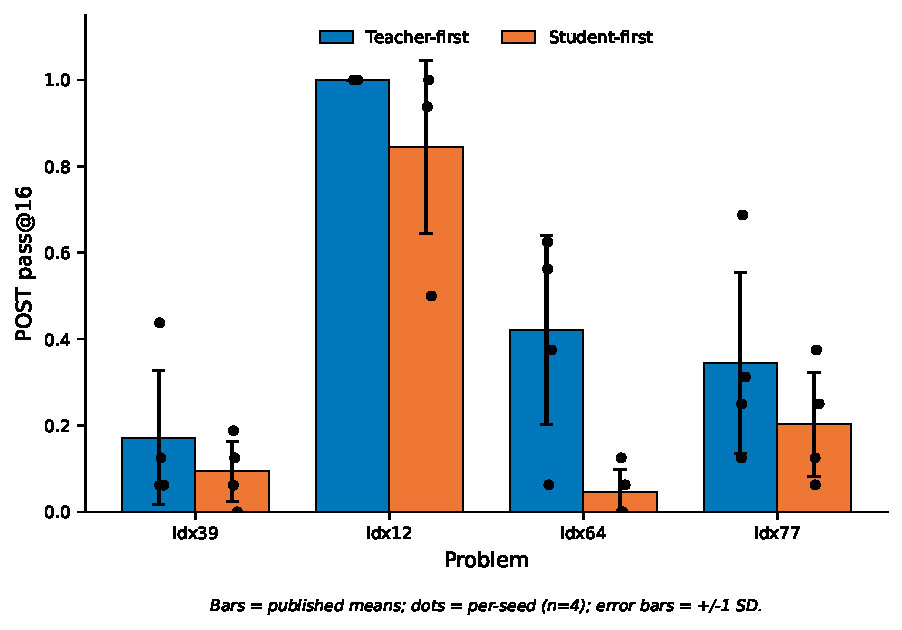
\includegraphics[width=0.85\linewidth]{../figures/fig_4_1_main_result.pdf}\end{center}

\textbf{Figure 4.1}
\emph{POST pass@16, teacher-first versus student-first.} Bars are the published means; dots are per-seed values (\(n=4\), all four problems, recovered and verified from the W\&B export); error bars are \(\pm 1\) SD. Teacher-first is at or above student-first on every problem.

\begin{center}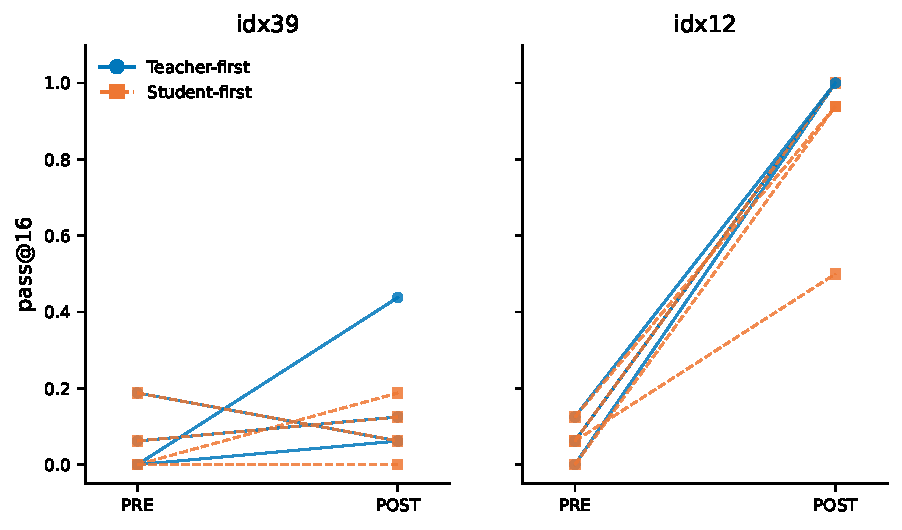
\includegraphics[width=0.85\linewidth]{../figures/fig_4_2_per_seed_slope.pdf}\end{center}

\textbf{Figure 4.2}
\emph{Per-seed PRE→POST change.} Each line is one seed. Teacher-first (solid) is at or above student-first (dashed) on every seed; teacher-first reaches 1.0 on all seeds of idx12 while student-first varies.

\subsection{4.2.3 Hard-frontier escape-zero}\label{hard-frontier-escape-zero}

The main result is weak dominance. The sharper claim comes from extending the matched comparison to harder, lower-pass problems, to test the flat-reward-trap hypothesis directly: on-policy SF should stay stuck at zero where the bare student rarely rolls a correct attempt, while TF escapes because the teacher can generate a correct solution to distill.

\begin{longtable}[]{@{}
  >{\raggedright\arraybackslash}p{(\columnwidth - 12\tabcolsep) * \real{0.1429}}
  >{\raggedright\arraybackslash}p{(\columnwidth - 12\tabcolsep) * \real{0.1429}}
  >{\raggedright\arraybackslash}p{(\columnwidth - 12\tabcolsep) * \real{0.1429}}
  >{\raggedright\arraybackslash}p{(\columnwidth - 12\tabcolsep) * \real{0.1429}}
  >{\raggedright\arraybackslash}p{(\columnwidth - 12\tabcolsep) * \real{0.1429}}
  >{\raggedright\arraybackslash}p{(\columnwidth - 12\tabcolsep) * \real{0.1429}}
  >{\raggedright\arraybackslash}p{(\columnwidth - 12\tabcolsep) * \real{0.1429}}@{}}
\toprule\noalign{}
\begin{minipage}[b]{\linewidth}\raggedright
problem
\end{minipage} & \begin{minipage}[b]{\linewidth}\raggedright
id
\end{minipage} & \begin{minipage}[b]{\linewidth}\raggedright
judge
\end{minipage} & \begin{minipage}[b]{\linewidth}\raggedright
SF mean
\end{minipage} & \begin{minipage}[b]{\linewidth}\raggedright
TF mean
\end{minipage} & \begin{minipage}[b]{\linewidth}\raggedright
win/tie/loss
\end{minipage} & \begin{minipage}[b]{\linewidth}\raggedright
escape-zero
\end{minipage} \\
\midrule\noalign{}
\endhead
\bottomrule\noalign{}
\endlastfoot
idx39 & abc393\_d & difflib & 0.094 & 0.172 & 2/2/0 & seed1 (SF 0→0, TF 0.062) \\
idx64 & abc397\_e & LLM-groq & 0.047 & \textbf{0.422} & 4/0/0 & seed1 (SF 0.062→0, TF 0.375), seed2 (SF 0→0, TF 0.062) \\
idx77 & abc399\_f & difflib & 0.203 & 0.344 & 3/1/0 & --- (SF not stuck at 0 here) \\
\textbf{total} & & & & & \textbf{9/3/0} & \textbf{3 instances / 2 problems} \\
\end{longtable}

Three findings. TF beats SF on all three hard problems and never loses; the crude sign test over the 9 non-tied pairs is \(0.5^9 \approx 0.002\). \textbf{Escape-zero replicates three times} (idx39 s1, idx64 s1 and s2): SF stays at or falls back to pass = 0 while TF escapes. This is the direct mechanistic signature predicted in §3.6: the on-policy flat-reward trap versus off-policy injection. idx64 is the strongest case, TF 0.422 versus SF 0.047 (roughly 9×), winning 4/4.

Two honest caveats. idx39 appears in both §4.2.2 and this table, so the two groupings are not independent. And the judge differs across problems (idx64 uses the LLM judge, idx39/77 use difflib), which is acceptable only because §4.4 separately establishes judge-invariance.

\begin{center}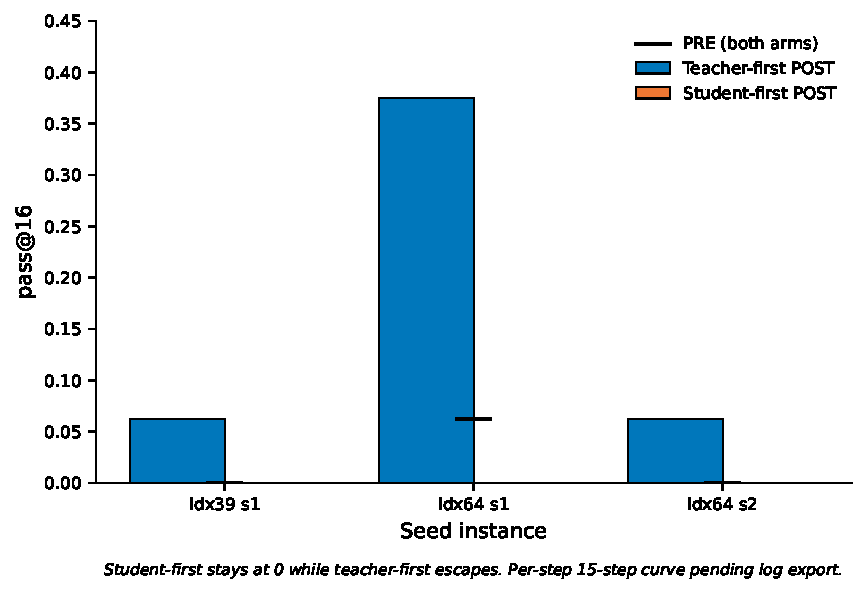
\includegraphics[width=0.85\linewidth]{../figures/fig_4_3_escape_zero.pdf}\end{center}

\textbf{Figure 4.3}
\emph{Escape-zero instances.} On three seeds, student-first POST stays at 0 (or falls back to it) while teacher-first lifts off zero. Black marks are PRE (shared by both arms). The per-step 15-step discovery curve is pending log export.

\begin{quote}
\textbf{Claim, calibrated.} The contribution is not ``TF wins by a small margin.'' It is: \emph{teacher-first learns on hard problems where on-policy SDPO is caught in a flat-reward trap, the margin is large, and escape-zero is replicated.} The claim is bounded by n: 2--3 problems, one 4B model, template T2, and no compute matching (TF generates roughly 2.5× more, so it wins on outcome, not yet on compute).
\end{quote}

\subsection{4.2.4 Discovery curves and qualitative behavior}\label{discovery-curves-and-qualitative-behavior}

Beyond aggregate pass-rate, the runs show genuine discovery rather than confidence inflation. On idx12, greedy decoding moves 0.075 → 1.0; on idx39, 0.175 → 0.225. The model learns to solve problems it deterministically failed before. One concrete trace (full excerpt in Appendix D.5): idx12 base uses \texttt{math.factorial(X)} in the wrong direction, the feedback reports a runtime error, and the model learns to iterate to find N. In an exploratory run (idx29), the base calls \texttt{exit()} (unavailable in the sandbox), the feedback reports a \texttt{NameError}, and the model corrects it.

Two further observations. On easy-to-fix exploratory problems (idx23, idx29 at eval-8), both arms solve almost equally, so differentiation is clearer on harder problems. And from around step 2 the teacher tends to converge (batch reward = 1.0, mean similarity ≈ 0.9, \texttt{n\_good} → 1); when the base starts high, both arms can over-distill, consistent with the idx39 seed-3 control above.

\subsection{4.2.5 Compute considerations (RQ3, partial)}\label{compute-considerations-rq3-partial}

The comparisons above are matched on seeds and on the step budget, but not on generations. Teacher-first draws \texttt{teacher\_n=10} samples per step against student-first's four, roughly a 2.5× generation overhead, so the results establish an outcome advantage rather than a compute-fair one. Two observations bound what can be said. The discovery curves (§4.2.4) show teacher-first reaching a high pass-rate within the 15-step budget, and the escape-zero seeds show student-first failing across its own 60 generations (4 per step over 15 steps) while teacher-first escapes. This points to the \emph{kind} of distilled trajectory, rather than raw sample volume, as the driver of the gap.

The point is suggestive, not conclusive. Student-first was never run at teacher-first's generation budget, and no best-of-k baseline was measured at matched compute, so more student-first sampling cannot be ruled out as an alternative route to escape. A full answer needs a compute-to-correct frontier that holds total generations fixed and logs token and GPU-time cost; §6.2.4 sets this out as future work. RQ3 is therefore answered only in part here: the overhead is quantified and the missing comparison is identified, but the Pareto trade-off itself is not measured.

\begin{center}\rule{0.5\linewidth}{0.5pt}\end{center}

\section{4.3 RQ1: the reprompt template}\label{rq1-the-reprompt-template}

RQ1 probes the titular question directly. Holding the SF arm fixed (script 07, Qwen3-4B, thinking OFF, 15 steps, eval-16), three templates were run on two problems at 2 seeds each. POST pass@16:

\begin{longtable}[]{@{}
  >{\raggedright\arraybackslash}p{(\columnwidth - 4\tabcolsep) * \real{0.3333}}
  >{\raggedright\arraybackslash}p{(\columnwidth - 4\tabcolsep) * \real{0.3333}}
  >{\raggedright\arraybackslash}p{(\columnwidth - 4\tabcolsep) * \real{0.3333}}@{}}
\toprule\noalign{}
\begin{minipage}[b]{\linewidth}\raggedright
Template
\end{minipage} & \begin{minipage}[b]{\linewidth}\raggedright
idx12 (easy)
\end{minipage} & \begin{minipage}[b]{\linewidth}\raggedright
idx39 (hard)
\end{minipage} \\
\midrule\noalign{}
\endhead
\bottomrule\noalign{}
\endlastfoot
T1\_minimal (``provide a corrected solution'') & 0.66 & \textbf{0.03} \\
T2\_standard (``correctly solve the original question'') & 0.97 & 0.06 \\
T5\_reasoning (``identify root cause, then provide corrected'') & 0.97 & \textbf{0.13} \\
\end{longtable}

On the hard problem the ordering is monotone, \textbf{T5 \textgreater{} T2 \textgreater{} T1} (0.13 \textgreater{} 0.06 \textgreater{} 0.03), and T5 is stable across its two seeds (.125 / .125). A reasoning-inducing reprompt beats the plain anchor, which beats the minimal one. On the easy problem T2 and T5 saturate together near 0.97 while T1 drops to 0.66 (partly one unlucky seed).

The template has an effect, and that effect is clearest on the hard problem where there is room to differentiate. This is directional evidence for RQ1, not a strong-power result: n = 2 seeds and the absolute counts are small. The probe is also on the SF arm only; the template × teacher-first interaction is left for future work (Chapter 6).

\begin{center}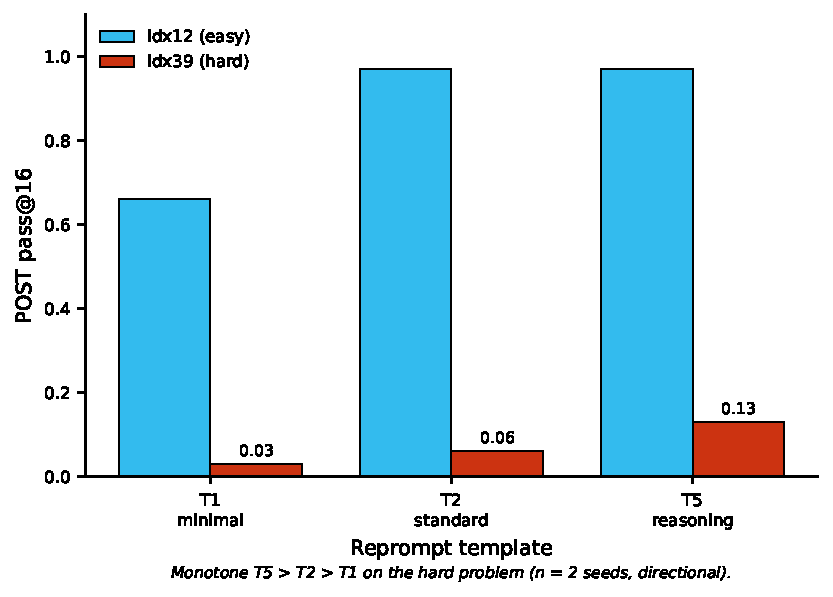
\includegraphics[width=0.85\linewidth]{../figures/fig_4_4_template.pdf}\end{center}

\textbf{Figure 4.4}
\emph{Reprompt-template effect on POST pass@16.} On the hard problem (idx39) the ordering is monotone T5 \textgreater{} T2 \textgreater{} T1; on the easy problem (idx12) T2 and T5 saturate. Directional only (\(n=2\) seeds).

\begin{center}\rule{0.5\linewidth}{0.5pt}\end{center}

\section{4.4 Robustness ablations}\label{robustness-ablations}

\subsection{4.4.1 Judge-invariance}\label{judge-invariance}

The independence judge can be a cheap string-similarity check (difflib) or a semantic LLM judge (groq \texttt{llama-3.3-70b}). Mean POST pass over 4 seeds, good\_only:

\begin{longtable}[]{@{}llll@{}}
\toprule\noalign{}
problem & SF & TF · difflib & TF · LLM \\
\midrule\noalign{}
\endhead
\bottomrule\noalign{}
\endlastfoot
idx39 & 0.094 & 0.172 & 0.266 \\
idx12 & 0.844 & 1.000 & 0.984 \\
\end{longtable}

TF ≥ SF under both judges on both problems, and the two judges give similar student POST, so the core result is \textbf{invariant to the judge choice}. The two judges do label differently: the semantic LLM calls fewer trajectories ``copy'' than difflib (on idx12 the LLM keeps \texttt{n\_good} up to 10 versus 1 for difflib), but the \emph{outcome} is unchanged, because the update is driven by correctness and convergence rather than by the exact copy boundary. As noted in §3.3.3, with thinking OFF the judge's \texttt{reasoning\_quality} saturates at 4--5, so it functions only as a copy-detector; no claim is made about reasoning quality.

\subsection{4.4.2 Leak ablation (good\_only vs good\_bad)}\label{leak-ablation-good_only-vs-good_bad}

Option 1 (good\_bad) feeds reference-like ``bad'' exemplars back to the teacher and so should leak if leak matters here; Option 2 (good\_only) does not. Mean POST pass, LLM judge:

\begin{longtable}[]{@{}lll@{}}
\toprule\noalign{}
arm & idx39 & idx12 \\
\midrule\noalign{}
\endhead
\bottomrule\noalign{}
\endlastfoot
SF baseline & 0.094 & 0.844 \\
TF · good\_only & 0.266 & 0.984 \\
TF · good\_bad & 0.250 & 1.000 \\
\end{longtable}

good\_bad ≈ good\_only (idx39 0.250 vs 0.266; idx12 1.000 vs 0.984). Showing the teacher labeled ``bad/copy'' exemplars does \textbf{not} change the result, so the advisor's information-leak concern does not materialize on this data. This is the predicted leak-null for code (§3.5): the reference is best-in-batch plus public tests, not an author solution, so there is little to leak. Against SF, good\_bad scores 7 wins / 1 tie / 0 loss (idx39 wins 4/4, cleaner than good\_only); crude sign test \(0.5^7 \approx 0.008\). This corroborates the main result without raising the claim, since it is still 2 problems.

\begin{center}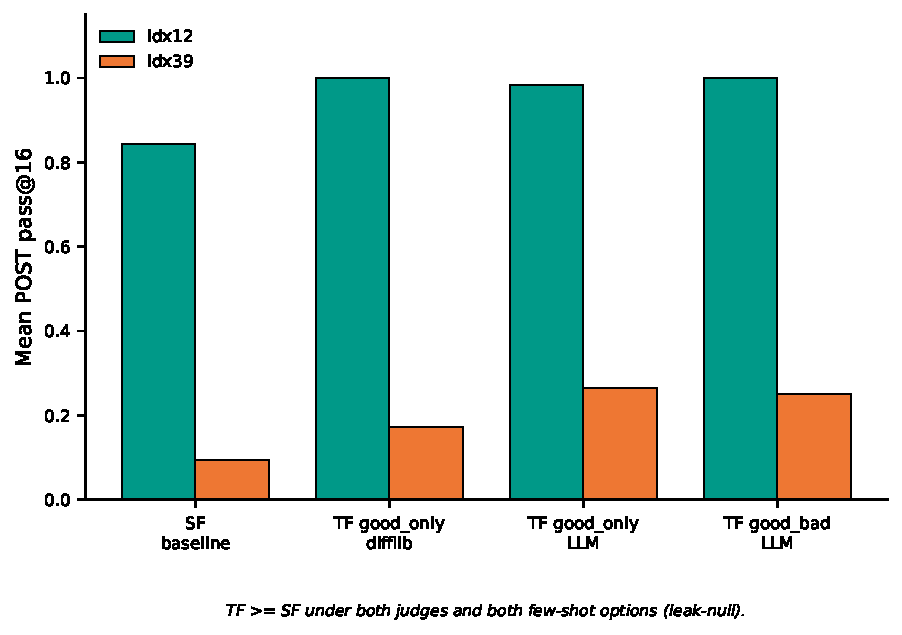
\includegraphics[width=0.85\linewidth]{../figures/fig_4_5_ablation.pdf}\end{center}

\textbf{Figure 4.5}
\emph{Judge × few-shot ablation, mean POST pass@16.} Teacher-first stays at or above the student-first baseline across both judges (difflib, LLM) and both few-shot options (good\_only, good\_bad); good\_bad ≈ good\_only indicates the leak is null on code.

\begin{center}\rule{0.5\linewidth}{0.5pt}\end{center}

\section{4.5 Math pilot: a boundary characterization}\label{math-pilot-a-boundary-characterization}

The math pilot extends the comparison to the domain where the advisor and Kim et al.~{[}2{]} expect leak and epistemic effects to be strongest. It is a pilot in the strict sense: 2 problems, a different model, and an answer-only reference (§3.5). It does not escape, and that non-escape is informative about \emph{when} teacher-first works.

\subsection{4.5.1 Setup and frontier scan}\label{setup-and-frontier-scan}

Gemma-4-E4B (thinking ON) on MathArena AIME 2026 {[}10{]} (30 problems, integer answers), \texttt{reference\_mode\ =\ ground\_truth} (the teacher always sees the correct answer, the extreme leak regime), LLM judge \texttt{glm-4.5-flash} with a derive-vs-copy prompt. A frontier scan (n\_samples = 2) spreads the problems out: frontier (0 \textless{} pass \textless{} 1) at idx 8, 11, 21, 25; too-hard (pass = 0) at 15 problems; ceiling (pass = 1) at 11 problems. Gemma-4 with thinking solves many AIME 2026 problems, so difficulty is scattered rather than monotone.

\begin{center}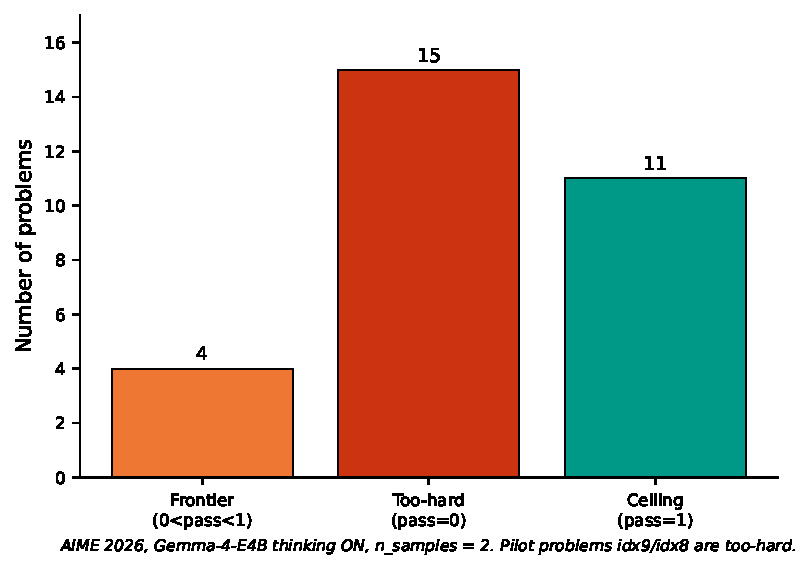
\includegraphics[width=0.85\linewidth]{../figures/fig_4_7_frontier_bands.pdf}\end{center}

\textbf{Figure 4.7}
\emph{AIME 2026 frontier-scan band membership.} Of 30 problems, 4 are frontier (0 \textless{} pass \textless{} 1), 15 too-hard (pass = 0), and 11 at ceiling (pass = 1). The two pilot problems (idx9, idx8) are drawn from the too-hard band.

\subsection{4.5.2 No escape on too-hard problems}\label{no-escape-on-too-hard-problems}

The first clean run, idx9 (triangle 13-14-15 rotated about the circumcenter, hexagon area, correct answer 156):

\begin{longtable}[]{@{}lll@{}}
\toprule\noalign{}
& PRE & POST \\
\midrule\noalign{}
\endhead
\bottomrule\noalign{}
\endlastfoot
pass\_rate & 0.000 & 0.000 \\
greedy & 0.000 & 0.000 \\
boxed answer & 148 & 168 \\
\end{longtable}

Discovery curve 1.00 → 1.00 → 1.00, with \texttt{n\_good=1,\ n\_bad=3} each step. Teacher-first does \textbf{not} pull the too-hard problem off zero. idx8 (a dice/sticker probability problem, correct answer 29) replicates this: labeled frontier by the noisy scan but actually PRE pass = 0 at 4 samples, PRE boxed 40201 → POST boxed 17, still wrong, PRE 0 → POST 0.

The reason is regime, not compute. With thinking ON and 16384 tokens (no truncation), the model reasons to completion and still answers wrong with confidence (148, 168). This rules out ``did not think enough'' and identifies a \textbf{capability ceiling}. Because the reference is only the number 156, the teacher can copy but has no in-reach method to distill, and distilling a few answer-aware traces cannot install a capability the model lacks. The code notion of ``hard'' is reachable-but-stuck (solvable once unblocked by feedback or best-in-batch); the AIME ``too-hard'' problems are beyond-capability. The wrong regime was selected, which is precisely the boundary the pilot characterizes.

\begin{center}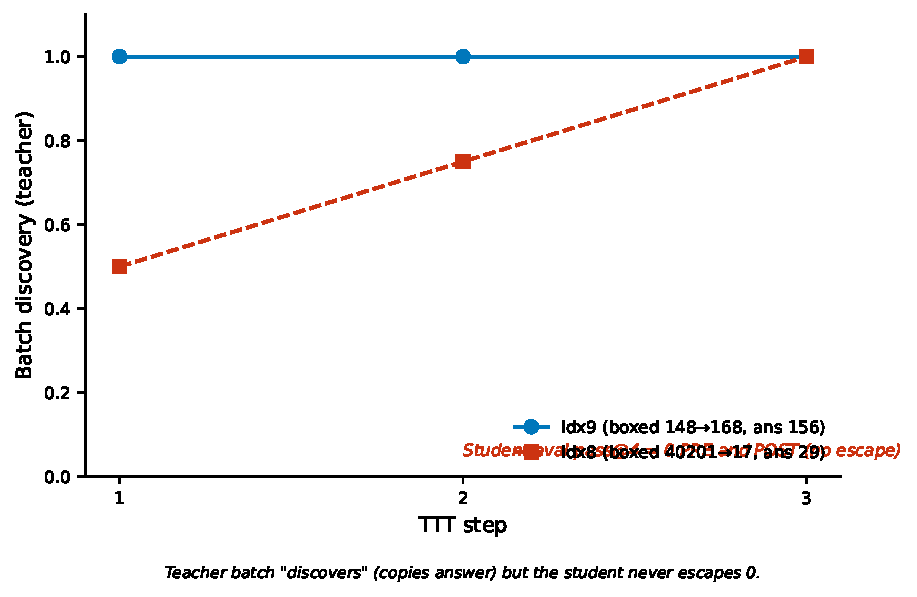
\includegraphics[width=0.85\linewidth]{../figures/fig_4_6_math_discovery.pdf}\end{center}

\textbf{Figure 4.6}
\emph{Math teacher-batch discovery versus student escape.} The teacher's batch ``discovers'' the answer across the three steps (it copies the leaked answer), yet the student's eval pass@4 stays at 0 both PRE and POST. The boxed answer drifts (148→168, 40201→17) without reaching the correct value, illustrating form changing while substance does not.

\subsection{4.5.3 Measured leak, and a fallback that defeats the judge}\label{measured-leak-and-a-fallback-that-defeats-the-judge}

Although the pilot does not escape, the judge measures the leak cleanly, which is an on-thesis positive. With the leaked answer 156, all four teacher trajectories are nominally ``correct'' every step (batch mean reward 1.0 across all three steps of idx9), yet the judge flags most of them as copies. Across the 12 judged trajectories (full verdict log in Appendix D):

\begin{longtable}[]{@{}
  >{\raggedright\arraybackslash}p{(\columnwidth - 4\tabcolsep) * \real{0.3333}}
  >{\raggedright\arraybackslash}p{(\columnwidth - 4\tabcolsep) * \real{0.3333}}
  >{\raggedright\arraybackslash}p{(\columnwidth - 4\tabcolsep) * \real{0.3333}}@{}}
\toprule\noalign{}
\begin{minipage}[b]{\linewidth}\raggedright
\end{minipage} & \begin{minipage}[b]{\linewidth}\raggedright
is\_copy = true (asserts 156)
\end{minipage} & \begin{minipage}[b]{\linewidth}\raggedright
genuine derivation (independent, rq ≥ 3)
\end{minipage} \\
\midrule\noalign{}
\endhead
\bottomrule\noalign{}
\endlastfoot
count (of 12) & \textbf{10 (≈83\%)} & \textbf{1} \\
\end{longtable}

The single genuine derivation appears only at step 1 (is\_copy=false, reasoning\_quality 4); at steps 2 and 3 every trajectory is a copy. The filter keeps one trajectory as good each step (\texttt{n\_good=1,\ n\_bad=3}), a 75\% per-step reject rate, but at steps 2--3 that one ``good'' is itself a copy retained by the keep-best-correct fallback (§3.3.3). So the privileged teacher mostly copies the answer rather than deriving it, the judge detects this, and this is measurable information leak, exactly the concern of {[}2{]} and the contrast with code, where leak is null (§4.4).

The idx8 log (run 463y4fjr) sharpens the second-order problem. There, \emph{every} judge verdict across all three steps is \texttt{is\_copy=true} (the single \texttt{is\_copy=false} has reasoning\_quality 2 \textless{} 3, so it is also bad). The \texttt{n\_good=1} per step therefore comes \emph{entirely} from the fallback: the good pool consists only of copies the judge already rejected. The fallback defeats the judge when the teacher produces nothing but copies. This is also a judge-degradation effect: the judge catches blatant copying but cannot reliably separate a genuine derivation from an answer-directed confabulation on beyond-capability problems, where both reach the right number.

\subsection{4.5.4 Epistemic pathology: form changes, substance does not}\label{epistemic-pathology-form-changes-substance-does-not}

Reading the full thinking traces shows what TTT actually transfers in the leak regime. The model satisfices toward a ``clean'' number: when stuck it assumes a value (PRE θ = 90°; POST Area = 2K = 168) and rationalizes it (``in problems of this nature, the intended answer is usually clean''), guessing by contest convention rather than deriving. It shows \textbf{epistemic suppression} {[}2{]}: it knows the problem is ambiguous (``this is impossible'', ``contradiction'') but does not admit it and emits a confident answer. It performs ``self-correction theater'', labeling steps ``Crucial Insight Check'' and ``Self-Correction'' while the correction loops without converging.

Most telling, POST is half the length (≈24k → 12k characters) with a better setup (it now knows cos C = 3/5, θ = 90° ± C) but gives up earlier and cuts a corner to a wrong answer (168). The student learns the teacher's \emph{confident reasoning style} from answer-aware traces but not its method. This is epistemic mimicry made visible: form transfers, substance does not. The model does not even memorize 156. idx8 runs the opposite direction (POST is \emph{more} rigorous, with casework) yet is still wrong, so TTT changes reasoning style in both directions without fixing correctness.

\subsection{4.5.5 Pilot conclusion}\label{pilot-conclusion}

Across two too-hard AIME problems, teacher-first does not escape, and the non-escape is consistent and interpretable: the teacher copies the answer (the judge catches roughly 75\%), the leak transfers form rather than substance (replicated across both problems), and the student stays at zero. Stated as a boundary: \textbf{teacher-first escapes when the reference provides an in-reach method (code, §4.2), and fails when the teacher has only the answer on a beyond-capability problem (AIME too-hard).} Escape requires reachable capability, not merely a correct answer. This contrast is stronger evidence about the mechanism than a ``works everywhere'' result would be.

\begin{center}\rule{0.5\linewidth}{0.5pt}\end{center}

\section{In-chapter citations}\label{in-chapter-citations}

Numbered per the master bibliography (\texttt{00\_references.md}): {[}1{]} Hübotter et al.~2026 · {[}2{]} Kim et al.~2026 · {[}7{]} Qwen3 · {[}10{]} MathArena AIME 2026. (Full method and metric definitions in Chapter 3.)
